% Use UTF-8 encoding!!
% (c) Stefan Ulbrich, 2012
% updated in May, 2015 by Michael Bechtel

\documentclass[english,ngerman]{KITreprt}


%% --------------------------------
%% Obligatory Parameters:
%% --------------------------------

%\renewcommand{\mythesis}{\termpaper} %\mastersthesis, \bachelorsthesis, \protocol, \studienarbeit, \diplomarbeit
\renewcommand{\mytitle}{ \iflanguage{english}{The KITreprt Class}{Die KITreprt Klasse} }
\renewcommand{\myname}{\textcolor{red}{Your Name}}
%\renewcommand{\myshorttitle}{Die offizielle \LaTeX-Vorlage des HIS}
\renewcommand{\myshorttitle}{}
\cfoot{\mytitle}

\renewcommand{\timestart}{4. November 2011}
\renewcommand{\timeend}{\iflanguage{english}{February 7\textsuperscript{th},}{7. Februar} 2010}
\newcommand{\referee}{Erstgutachter}
\newcommand{\refereetwo}{Zweitgutachter}
%\newcommand{\refereethree}{Drittgutachter}

\newcommand{\advisor}{Betreuender Mitarbeiter 1}
\newcommand{\advisortwo}{Betreuender Mitarbeiter 2}
%\newcommand{\advisorthree}{Betreuender Mitarbeiter 3}

\graphicspath{{./images/}}


%% -------------------------------
%% |  Information for PDF file   |
%% -------------------------------
\hypersetup{
	pdfauthor={\myname},
	pdftitle={\mytitle},
	pdfsubject={Not set},
	pdfkeywords={Not set}
}




\begin{document}


\selectlanguage{ngerman}
%\selectlanguage{english}


\maketitle

\thispagestyle{empty}
\newpage
%\topskip0pt
\vspace*{\fill}
\noindent
\textbf{Erkl\"arung:}\\
\\
\noindent
Ich versichere hiermit, dass ich die Arbeit selbstst\"andig verfasst habe, keine anderen als die angegebenen Quellen und Hilfsmittel benutzt habe, die w\"ortlich oder inhaltlich \"ubernommenen
Stellen als solche kenntlich gemacht habe und die Satzung des Karlsruher Instituts f\"ur Technologie zur Sicherung guter wissenschaftlicher Praxis beachtet habe.\\
\\
\\
\noindent
Karlsruhe, den \timeend 
\begin{flushright}

\myname
\end{flushright}

\vspace*{\fill}
\cleardoublepage



\thispagestyle{empty}
\newpage
%\topskip0pt
\vspace*{\fill}
\noindent
\textbf{Abstract:}\\
\\
\noindent
English abstract goes here.
\vspace*{\fill}
\cleardoublepage


\thispagestyle{empty}
\newpage
%\topskip0pt
\vspace*{\fill}
\noindent
\textbf{Kurzzusammenfassung:}\\
\\
\noindent
Deutsche Kurzzusammenfassung hier.
\vspace*{\fill}
\cleardoublepage


\tableofcontents
\setcounter{page}{1}
\chapter{Erstellung studentischer wissenschaftlicher Arbeiten mit der \emph{KITreprt}-Klasse} 

Die \emph{KITreprt}-Klasse dient vorrangig der Erstellung studentischer wissenschaftlicher Texte wie zum Beispiel Bachelor- oder Masterarbeiten. 
Aufbauend auf dem \emph{Koma-Script}\footnote{\url{http://www.komascript.de/}} bietet diese Klasse eine KIT-konforme Titelseite, bindet die empfohlenen Pakete
standardm\"a{\ss}ig ein und versucht ein m\"oglichst ansprechendes Seitenlayout zu erzeugen.
In diesem Kapitel werden die Aspekte dieser Klasse vorgestellt und ein paar generelle Hinweise zur Verwendung von {\LaTeX} aufgezeigt.
Dieses Dokument wurde mit dieser Klasse erstellt und der Quelltext soll als weiterf\"uhrendes Beispiel  dienen.

\section{Die \emph{KITreprt}-Klasse}
\subsection{Verwendung der Klasse}
Die Klasse wird mit dem Befehl \lstinline[language={[LaTeX]TeX}]!\documentclass[english,ngerman]{KITreprt}! eingebunden.
Die Sprache kann mit den Befehlen \lstinline[language={[LaTeX]TeX},morekeywords={selectlanguage}]!\selectlanguage{ngerman}! und \lstinline[language={[LaTeX]TeX},morekeywords={selectlanguage}]!\selectlanguage{english}! zwischen dem Deutschen und dem Englischen umgeschalten werden.
Dokumente mit der \emph{KITreprt}-Klasse sollten direkt mit \emph{Pdflatex} in Pdf-Dokumente \"ubersetzt werden und unbedingt \emph{UTF-8} als Zeichenkodierung verwenden.

%\begin{tikzpicture}[remember picture,x=\textwidth,y=\textheight,yscale=-1.0,overlay,shift=(current page text area.north west)]
%    \draw[thick,red] (0,0) rectangle (1,1);
%\end{tikzpicture}

    
\subsection{Die Einrichtung der Titelseite}
Das Layout der Titelseite ist komplett in der Klassendefinition enthalten und es werden keine weiteren Dateien, zum Beispiel f\"ur das Logo, ben\"otigt.
F\"ur die Daten auf der Titelseite m\"ussen \TeX-Makros definiert (bzw. neu definiert werden).
Sind diese nicht gesetzt erscheinen auf der Titelseite in roter Schrift Anweisungen, wie diese gesetzt werden m\"ussen.
Um ein Makro neu zu definieren reicht zum Beispiel die Anweisung \lstinline[language={[LaTeX]TeX}]!\renewcommand{\myshorttitle}{Die offizielle HIS-\LaTeX-Vorlage}!.
Die m\"oglichen Makros sind in Tabelle~\ref{tab:makros} aufgelistet.
Eine Ausnahme bilden die Makros \texttt{\textbackslash  advisor}, \texttt{\textbackslash  advisortwo}, \texttt{\textbackslash  reviewer} und \texttt{\textbackslash  reviewertwo}. 
Dies m\"ussen mit \texttt{\textbackslash  newcommand} komplett neu definiert werden, um auf der Titelseite zu erscheinen.
Ist keines dieser vier Makros definiert, muss ein spezielles Makro definiert werden, damit kein roter Text zu sehen ist:  \lstinline[language={[LaTeX]TeX}]!\renewcommand{\noadvisors}{}!.
\begin{table}[h]
\centering
\begin{tabular}{cl}
\toprule
Makro & Inhalt \\
\midrule 
\texttt{\textbackslash myname} & \emph{Name des Autors} \\
\texttt{\textbackslash mythesis} & \emph{Vordefiniert (zweisprachig):} \texttt{\textbackslash termpaper} \emph{(Seminararbeit)}, \texttt{\textbackslash mastersthesis}, \\
&  \texttt{\textbackslash bachelorsthesis}, \texttt{\textbackslash protocol},  \texttt{\textbackslash studienarbeit}, \\
& \texttt{\textbackslash diplomarbeit}, \emph{oder eigene Bezeichnung} \\
\texttt{\textbackslash myshorttitle} & \emph{Name der Arbeit} \\
\texttt{\textbackslash mytitle} & \emph{Optionaler Untertitel oder leer } \\
\texttt{\textbackslash timestart} & \emph{Anfangsdatum} \\
\texttt{\textbackslash timestart} & \emph{Datum der Abgabe} \\
\texttt{\textbackslash  advisor} & \emph{Name des betreuenden Mitarbeiteiters (Seminararbeiten)} \\
\texttt{\textbackslash  reviewer} & \emph{Name des Referenten} \\
\bottomrule
\end{tabular}
\caption{Die Makros die f\"ur die Titelseite definiert werden m\"ussen. Tabellen in wissenschaftlichen Texten sollten nach M\"oglichkeit nie vertikale Linien verwenden. }
\label{tab:makros}
\end{table}

\subsection{Vordefinierte Pakete }
Die folgenden Pakete werden in der \emph{KITreprt}-Klasse definiert und m\"ussen daher nicht von Hand eingebunden werden.
\begin{description}
\item[\emph{babel}] Lokalisierte Trennung und Schriftsatz. 
\item[\emph{fontenc}] Umlaute und Sonderzeichen.
\item[\emph{inputenc}] \emph{Utf-8} Zeichenkodierung. Dokumente m\"ussen diese Kodierung verwenden, um mit der Klasse verwendet werden zu k\"onnen.
\item[\emph{graphicx}] F\"ur die Einbindung von Graphiken in moderenen Formaten.
\item[\emph{amsmath,amssymb,amsthm}] Mathematische Symbole und Extrapakete.
\item[\emph{color}] F\"ur farbigen Text. Die Farbe \gqq{grey} wird auch in der Klasse definiert.
\item[\emph{subfigure}] Mehrere Einzelbilder in der selben Abbildung.
\item[\emph{booktabs}] Ansprechende Tabellen (siehe~Tab.~\ref{tab:makros}).
\item[\emph{listings}] Darstellung von Quelltexten (siehe Abschnitt~\ref{sec:code}).
\item[\emph{helvet,courier,mathptmx}] Alternative Schriften (z.B. Serifenlose Schrift f\"ur \"Uberschriften.
\item[\emph{lastpage}] Erlaubt die letzte Seite zu referenzieren
\item[\emph{natbib}] Paket zum Zitieren für die Naturwissenschaften. Der Stil \emph{abbrvnat} ist voreingestellt.
\item[\emph{tikz,eso-pic,setspace,automark}] Pakete, die intern zum Beispiel f\"ur die Titelseite verwendet werden.
\end{description}

\subsection{\LaTeX-Befehle}

Dieses Dokument soll nicht als ausf\"uhrliche Einf\"uhrung in \LaTeX verstanden werden.
F\"ur eine \"Ubersicht \"uber alle Befehle, wie zum Beispiel\lstinline[language={[LaTeX]TeX}]!\emph! f\"ur hervorgehobenen Text, wird daher auf folgende Quellen verwiesen:
\begin{itemize}
\item Die deutsche \href{http://de.wikipedia.org/wiki/LaTeX}{Wikipedia-Seite zu \LaTeX}\footnote{http://de.wikipedia.org/wiki/LaTeX} verweist auf einige gute Einf\"uhrungen.
\item Der \LaTeX Companion von \citet*{latexcompanion}.
\end{itemize}



\section{Verweise und Zitate}
\subsection{Verweise}
\label{sec:ref}
Um auf Stellen im selben Dokument zu verweisen wird der \lstinline[language={[LaTeX]TeX}]!\ref!-Befehl verwendet.
Dazu m\"ussen an den Betreffenden Stellen Markierungen (sogenannte Labels) mit dem\lstinline[language={[LaTeX]TeX}]!\label!-Befehl gesetzt werden.
\"Ublicherweise werden so Textstellen wie Kapitel und Abschnitte oder Abbildungen und Tabellen markiert.
Bei Textstellen k\"onnen direkt nach dem entsprechenden Befehl die Markierungen gesetzt werden, bei Abbildungen sowie Tabellen muss dies nach dem Festlegen der \"Uberschrift passieren. 
Die Verweise k\"onnen von \LaTeX erst nach wiederholtem \"Ubersetzen korrekt aufgel\"ost werden.
Es empfiehlt sich die Markierungsbezeichnungen zu strukturieren, zum Beispiel alle Abbildungen mit einem vorausgehenden \emph{fig:} zu kennzeichnen.
\subsection{Zitate}
F\"ur das Zitieren soll unbedingt \emph{Bibtex}\footnote{Weitere Informationen unter \url{http://www.bibtex.org/de/}} verwendet werden.
Das \emph{natbib}-Paket\footnote{\url{http://www.ctan.org/pkg/natbib}} stellt zus\"atzliche Befehle zum Zitieren zur verf\"ugung:
\begin{description}
\item[\texttt{citet}] Dieser Befehl erzeugt Zitate, die direkt im Text erscheinen: \citet{Asfour2006}, 
\item[\texttt{citet}$\ast$] Das Asterisk l\"asst alle Koautoren erscheinen: \citet*{Asfour2006}
\item[\texttt{citep}] Mit diesem Befehl werden Zitate in Klammern angezeigt: \citep{Asfour2006}
\end{description}
\emph{Wichtig:} Nicht nur direkte Zitate, die in Anf\"uhrungszeichen (im Deutschen der Befehl \lstinline[language={[LaTeX]TeX}]!\gqq!) gekennzeichnet werden m\"ussen, sondern auch alle Gedanken, Ideen oder Ans\"atze,
die nicht vom Autor stammen m\"ussen korrekt und vollst\"andig zitiert werden.
\subsection{Zeilenumbr\"uche}
Die \emph{cite}- und \emph{ref}-Befehle sollten immer durch eine vorangestellte Tilde ($\sim$) -- das steht in \LaTeX{} ein gesch\"utztes Leerzeichen -- direkt mit vorhergehenden Wort verbunden werden, damit kein unerw\"unschter
Zeilen- oder Seitenumbruch dazwischen erfolgen kann.\\
Zum Beispiel: \lstinline[language={[LaTeX]TeX},morekeywords={citep}]! Der Roboter Armar-III~\citep{Asfour2006} hat sieben Freiheitsgrade pro Arm.!

\section{Bilder und Tabellen}
In \LaTeX sollten Bilder und Tabellen prinzipiell nicht an einer festen Stelle an den Text gekoppelt werden.
Vielmehr gibt es daf\"ur Umgebungen (sogenannte \emph{floating}-Umgebungen), die die Bilder automatisch in der Nähe und an typographisch sinnvoller Stelle platzieren. 
F\"ur Abbildungen steht daf\"ur die \emph{figure-} und f\"ur Tabellen die \emph{tabular-}Umgebung zur Verf\"ugung. 
\subsection{Bilder}
Die Verwendung der \emph{figure}-Umgebung soll hier anhand eines kurzen Beispiels in Listing~\ref{lst:float} erl\"autert werden.
Die resultierende Abbildung ist Abb.~\ref{fig:example}.

\begin{center}
\begin{minipage}{0.65\textwidth} 
\begin{lstlisting}[language={[LaTeX]TeX},caption={Beispiel f\"ur eine Floatumgebung.},morekeywords={subfigure,includegraphics},label={lst:float}]
\begin{figure}[htbp]
\begin{center}
% Die beiden Teilbilder
\subfigure[Die humanoiden Roboter ARMAR-IIIa und ARMAR-IIIb am His.]{
\label{fig:example2a}
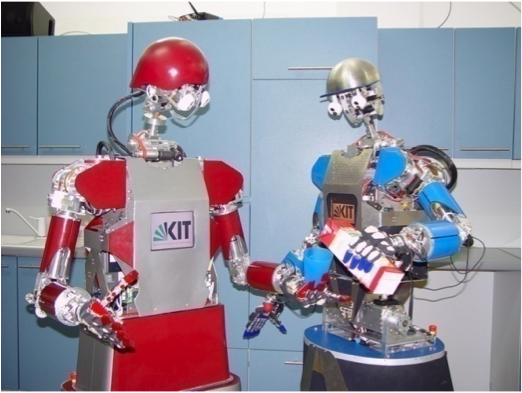
\includegraphics[width=0.3\textwidth]{Example1}}    
% horizontaler Abstand  von 1cm.
\hspace{1cm}            
\subfigure[Der Kopf des Roboters ARMAR-IIIa]{
\label{fig:example2b}
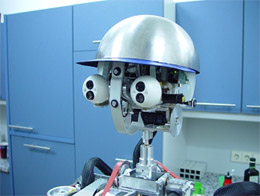
\includegraphics[width=0.3\textwidth]{Example2}}                
% Ueberschrift und Verweismarke fuer die gesamte Abbildung.
\caption{Die Roboter des HIS.}
\label{fig:example}
\end{center}
\end{figure}
\end{lstlisting}
\end{minipage}
\end{center}

\begin{figure}[htbp]
\begin{center}
\subfigure[Die humanoiden Roboter ARMAR-IIIa und ARMAR-IIIb am HIS.]{\label{fig:example2a}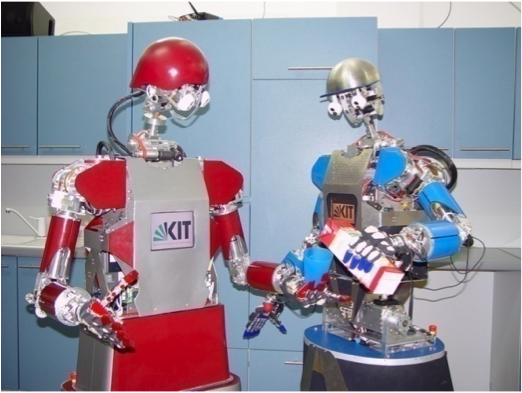
\includegraphics[width=0.3\textwidth]{Example1}}    
\hspace{1cm}            
\subfigure[Der Kopf des Roboters ARMAR-IIIa]{\label{fig:example2b}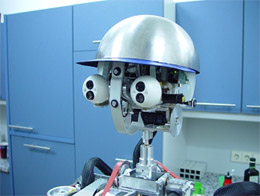
\includegraphics[width=0.3\textwidth]{Example2}}                
\caption{Die Roboter des HIS.}
\label{fig:example}
\end{center}
\end{figure}


Die eckigen Klammern umfassen die optionalen Parameter, die die Platzierung der Abbildung (nicht zwingend) beeinflussen. 
Die Parameter sind Pr\"aferenzen und \LaTeX{} versucht sie der Reihe nach zu erf\"ullen:
\begin{description}
\item[h] Direkt an der Stelle, wo es definiert wurde.
\item[t] Oben, am Anfang der Seite.
\item[b] Unten, am Ende der Seite.
\item[p] Gesondert, auf einer Extraseite f\"ur Abbildungen.
\end{description}
In der Umgebung ist eine \emph{center}-Umgebung eingeschlossen, die das Bild zentriert erscheinen l\"asst. 
Die beiden \emph{subfigure}-Befehle erzeugen die Einzelbilder der Abbildung.
Die optionalen Parameter in eckigen Klammern erzeugen die Bildunterschriften der Einzelbilder.
Gefolgt in den geschweiften Klammern k\"onnen Markierungen f\"ur Verweise auf die Einzelbilder angelegt werden (z.B. f\"ur Abb.~\ref{fig:example2a})
und mittels \texttt{\textbackslash includegraphics} wirklich die Graphikdatei in das Dokument eingebunden werden.
Wenn das Bild im Suchpfad liegt (siehe unten) ist keine vorangehende Pfadangabe und Dateierweiterung n\"otig. 
Der \emph{caption}-Befehl weiter unten erlaubt eine \"Uberschrift f\"ur die gesamte Abbildung anzugeben.
Die Markierung mittels \emph{label} wird in Abschnitt~\ref{sec:ref} behandelt.
Die ge\"offneten Umgebungen m\"ussen mit einem \emph{end} wieder geschlossen werden.
Anstelle der \emph{subfigure}-Befehle kann auch ein einzelnes \emph{includegraphics} stehen.
Der Graphikpfad kann wie folgt gesetzt werden (man beachte die doppelten geschweiften Klammern und dass die Anweisung vor dem Dokumentanfang stehen muss):\\
\lstinline[language={[LaTeX]TeX}]!\graphicspath{{./images/}}!


\subsection{Tabellen}
Die Umgebung f\"ur Tabellen \"ahnelt stark derer f\"ur Bilder -- inklusive \"Uberschriften und Textmarken.
Leider sind die Tabellen selbst relativ kompliziert in \LaTeX.
Daher wird an dieser Stelle auf den Quelltext dieses Dokuments und andere Quellen verwiesen\footnote{\url{http://en.wikibooks.org/wiki/LaTeX/Tables}}.
In Tabellen sollten generell vertikale Linien vermieden werden, um ein modernes Erscheinungsbild zu garantieren.
Das \emph{booktabs}-Paket\footnote{\url{http://ctan.org/tex-archive/macros/latex/contrib/booktabs/}} erm\"oglicht hier die Verwendung unterschiedlich dicker Linien mit \texttt{\textbackslash toprule},
\texttt{\textbackslash midrule} und \texttt{\textbackslash bottomrule} (siehe Tab.~\ref{tab:makros}). 


\section{Quelltexte}\label{sec:code}
Um Quelltexte (engl. Listings) wie in Listing~\ref{lst:float} zu setzen sollte das \emph{listings}-paket\footnote{\url{http://www.ctan.org/tex-archive/macros/latex/contrib/listings/}} verwendet werden.
Listings in \emph{float}-Umgebungen werden mit abgerundeten Rahmen gem\"ass der Titelseite versehen und unterst\"utzen Syntaxhighliting (farbliche Kennzeichnung von Spracheigenheiten).
Als Standard-Sprache ist nach einbinden der Klasse \emph{C++} voreingestellt.

So kann man zum Beispiel mit \lstinline[language={[LaTeX]TeX}]-\lstinline[language={[LaTeX]TeX}]!\emph!- \LaTeX-Befehle im Text eingebettet anzeigen.
F\"ur weitere Beispiele sollte der Quelltext dieses Dokuments untersucht werden.

\begin{equation}
e^x = \frac{e^{2\dot x} }{ \| x \|}
\end{equation}

%
%\chapter{Hinweise f\"ur studentische Hilfswissenschaftler}
%
%In diesem Kapitel werden einige Themen, die f\"ur die Arbeit an den \emph{Humanoids and Intelligence Systems Laboratories} wichtig sind, vorgestellt. 
%Die Themen umfassen Bereiche wie Programmiersprachen, Versionsverwaltung und den Webservices, die f\"ur die Arbeit am Institut n\"utzlich sind. 
%Diese kurze \"Ubersicht soll nur den Einstieg in die Materie vereinfachen verweist auf weiterf\"uhrende Literatur.
%
%
%\section{C++ Templates}
%\subsection{Generische Programmierung -- Quelltexterzeugung durch Schablonen}
%\begin{center}
%\begin{minipage}{0.5\textwidth}
%\begin{lstlisting}[caption={Eine einfache \textit{Tupel-}Klasse f\"ur den Datentyp \textit{double}.},label={lst:doubletupel}]
%class DoubleTupel {
%private: 
%  double a[2];
%public: 
%  DoubleTupel(double[])
%  {...};
%  double add(){ 
%    return a[0]+a[1];
%  };     
%};
%\end{lstlisting}
%\end{minipage}
%\hfill
%\begin{minipage}{0.45\textwidth}
%\begin{lstlisting}[boxpos=c,caption={Eine einfache \textit{Tupel-}Klasse f\"ur den Datentyp \textit{int}.},label={lst:inttupel}]
%class IntTupel {
%private: 
%  int a[2];
%public: 
%  DoubleTupel(int[])
%  {...};
%  int add(){ 
%    return a[0]+a[1];
%  };     
%};
%\end{lstlisting}
%\end{minipage}
%\end{center}
%
%Wenn noch verlangt wird, dass es Tupel mit unterschiedlicher Anzahl Elemente f\"ur jeden Datentyp existieren sollen, so explodiert die Anzahl der m\"oglichen Kombinationen. 
%Es w\"are deswegen w\"unschenswert, dass ein Mechanismus existierte, der genau diese Kombinationen anhand einer Schablone (engl. template) generiert.
%Genau diese Funktion gibt bereits in C++\footnote{Diese Mechanismen existieren unter dem Begriff \textit{generics} ebenfalls in anderen Sprachen wie C\# und Java (ab Version 5)}.
%Mit Hilfe des \texttt{templates} Schl\"usselwortes lassen sich genau solche Schablonen erzeugen.
%Ein Tupel, das solch einer Schablone (siehe Listing~\ref{lst:templatetupel}) entspricht kann nun einfach durch die Angabe des Datentyps und der Anzahl der Elemente erzeugt werden (Listing~\ref{lst:usetupel}).
%Man beachte, dass den Parametern der Schablone \textit{(engl. template parameters)} Standardwerte zugewiesen werden k\"onnen (im Beispiel die Anzahl der Elemente).
%\begin{center}
%%\begin{tabular}{b{0.5\textwidth}b{0.45\textwidth}}
%\begin{minipage}{0.5\textwidth}
%\begin{lstlisting}[caption={Eine Schablone f\"ur die \textit{Tupel-}Klassen.},label={lst:templatetupel}]
%template<typename T,
%int size=2>
%class Tupel {
%private: 
%  T a[size];
%public: 
%  T Tupel(T[])
%    {...};
%  T add(){ 
%    T sum = T[0];
%    for (int i=1;i<size;i++)
%      sum=sum+a[i];
%  };     
%};
%\end{lstlisting} 
%\end{minipage} \hfill
%\begin{minipage}{0.45\textwidth}
%\vspace{3.8cm} %unfortenately the only way to align captions - try and error
%\begin{lstlisting}[caption={Verwendung der Schablone.},label={lst:usetupel}]
%int main() {
%  Tupel<double,4> vierer;
%  Tupel<int> zweier;
%}; 
%\end{lstlisting}
%\end{minipage}
%%\end{tabular}
%
%\end{center}
%
%\paragraph{Achtung!}
%Wird die \textit{Tupel-}Klasse  f\"ur einen Datentyp erzeugt, f\"ur den der Operator \glqq+\grqq~ nicht definiert ist (zum Beispiel f\"ur Zeichenfolgen), f\"uhrt dies zu einer schwer zu verstehenden Fehlermeldung des Compilers.
%Als Ursprung des Fehlers wird insbesondere nicht die Erzeugung der Klasse mit einem ungeeigneten Parameter sein, sondern die Zeile an der die Addition stattfindet.
%Gerade wenn die Schablonen von jemand Anderem verfasst wurden, ist dann der Fehler nur sehr schwer zu finden.
%
%Eine weitere Einschr\"ankung stellt die Tatsache dar, dass Schablonen (entgegen der Spezifikation) bei allen \"ublichen Compilern \textit{komplett} in einer Header-datei definiert werden m\"ussen. 
%
%\subsection{Wichtige Templates des C++-Standards}
%
%Im C++-Standard (bzw. in den Standardbibliotheken) finden sich eine Reihe n\"utzlicher Klassen, die sich die M\"oglichkeiten des generischen Programmierens zunutze machen.
%In diesem Abschnitt werden zwei der gebr\"auchlichsten vorgestellt: \textit{vector} und \textit{map}.
%Bei beiden handelt es sich um so genannte Containerklassen, d.h. sie k\"onnen Objekte anderer Datentypen aufnehmen -- ganz wie die \textit{Tupel-}Klasse im letzten Abschnitt.
%Beide Klassen sind in dem Kontext \textit{(engl. namespace)} \glqq std::\grqq~  definiert, das bedeutet damit der Compiler die Namen richtig aufl\"osen kann, muss entweder \lstinline!std::! vor den Bezeichner gesetzt werden oder der aktuelle Kontext zum Beispiel mit 
%\lstinline!using namespace std;! erweitert werden.
%\paragraph{Die \textit{vector}-Klasse} kann wie ein dynamisch wachsendes Datenfeld \textit{(engl. array)} oder ein Stapel \textit{(engl. Stack)} verwendet werden.
%Um die Klasse zu verwenden muss die Klassendeklaration mittels \lstinline+#include <vector>+ eingebunden werden.
%\paragraph{Die \textit{map}-Klasse} stellt ein  \href{http://de.wikipedia.org/wiki/Assoziatives_Array}{assoziatives Array} zur Verf\"ugung.
%Damit kann einem Elements oder \glqq Schl\"ussel \grqq eines beliebigen Datentyps (wobei alle Schl\"ussel des selben Typs sein m\"ussen)  ein Element eines anderen Datentyps zugeordnet werden.
%Zum Beispiel lassen sich auf diese Weise dynamische Felder erzeugen deren Elemente mit Namen (\textit {string}-Objekten) adressiert werden k\"onnen. 
%
%\par Des Weiteren gibt es in den Standardbibliotheken n\"utzliche Klassen, wie zum Beispiel Sortieralgorithmen f\"ur die Containerklassen und die Stringklasse \textit{std::string}, die die veralteten C-Strings ersetzen soll. Die in C \"ubliche \textit{printf()} Funktion sollte durch das Objekt \textit{std::cout} ersetzt werden.
%
%\begin{center}
%\begin{minipage}{0.5\textwidth}
%\vspace{2.5\baselineskip}
%\begin{lstlisting}[caption={Die \textit{vector-}Klasse.},label={lst:vector}]
%#include <vector>
%#include <iostream>
%int main() {
%  using namespace std;
%   vector<int> v;
%  v.push_back(1);
%  v.push_back(12);
%  cout << "1: " << v[0] 
%    << "2:" << v[1] << endl;
%}
%\end{lstlisting}
%\end{minipage}
%\hfill
%\begin{minipage}{0.45\textwidth}
%\begin{lstlisting}[boxpos=b,caption={Die \textit{map-}Klasse.},label={lst:map}]
%#include <map>
%#include <string>
%#include <iostream>
%int main() {
%  std::map<char,int> m;
%// F\"uge der map Elemente 
%  // hinzu:
%  m['a']=1;
%  m['b']=5;
%  cout << "a: " << m['a'] 
%    << "b: " << m['b'] 
%    << endl;
%}
%\end{lstlisting}
%\end{minipage}
%\end{center}
%
%\subsection{Zuk\"unftige Erweiterungen und die Boost-Bibliotheken}
%Die \emph{Boost}-Bibliotheken\footnote{\url{http://www.boost.org/}} haben das Ziel den Funktionsumfang der Standardbibliotheken dem anderer moderner Programmiersprachen wie Java, C\# oder Python anzugleichen.  
%Ein Komitee entscheidet in einem strengen Prozess zur Qualit\"atssicherung dar\"uber, welche Bibliotheken zu Boost hinzugef\"ugt werden.
%Ein Gro{\ss}teil dieses Komitees ist dar\"uber hinaus an der Verabschiedung des neuen C++-Standards C++-11 beteiligt gewesen, so dass viele der Boost-Bibliotheken in den neuen Standard \"ubernommen wurden.
%Von den Bibliotheken werden zur Zeit unter Anderem folgende Bereiche abgedeckt: die Verarbeitung von Zeichenketten, weitere Container-Klassen, Algorithmen, funktionale Programmierung ($\lambda$-Kalk\"ul), Nebenl\"aufigkeit,
%Datenstrukturen, Ein- und Ausgabe, Bildverarbeitung und mehr.
%Wie bei den Standardbibliotheken sind die Funktionen in einem gesonderten Kontext \lstinline+boost::+ gesammelt.
%Eine sehr gute deutschsprachige Einf\"uhrung kann man im Internet\footnote{unter \url{http://www.highscore.de/cpp/boost/titelseite.html}} finden.
%
%\paragraph{Die \textit{boost::shared\_ptr}-Klasse} 
%Im Gegensatz zu Java oder C\# weisst C++ keine automatische Speicherverwaltung auf. Die Lebensdauer eines Objektes wird nur dann automatisch festgelegt, wenn es auf dem Stack angelegt wird (d.h. ohne die Verwendung von \textit{new}) und zwar genau dann wenn sein G\"ultigkeitsbereich verlassen wird.  \\
%Objekte, die mit \textit{new} erzeugt wurden, existieren bis der \textit{delete}-Operator auf sie angewendet wird.
%Dies hat kann zwei Probleme zur Folge haben.
%Zum einen m\"ussen alle Objekte die mittels \textit{new} angelegt werden auch wirklich von Hand mit \textit{delete} gel\"oscht werden um Speicherlecks zu verhindern.
%Zum anderen sind die Folgen wenn man umgekehrt versucht auf ein Objekt zu zugreifen, dass bereits nicht mehr existiert, gravierend.
%Es wird in diesem Fall keine Ausnahme \textit{(engl. exception)} ausgel\"ost wie bei den meisten modernen Sprachen.
%Anstelle dessen erfolgt meist eine unerlaubte Speicherzugriffsverletzung, die das sofortige Beenden des Programms ohne jeglichen Hinweis auf die Stelle des Fehlers zur Folge haben, oder  es gar k\"onnen Daten ausgelesen werden, die zu einem v\"ollig anderen Datenblock geh\"oren. 
%Die Klasse \textit{boost::shared\_ptr}, die mit  \lstinline+#include <boost/shared_ptr.hpp>+ verwendet werden kann, erg\"anzt C++ um einen Mechanismus, der genau solche Fehler verhindern soll.
%Dazu wird anstelle normaler Zeiger die Klasse \textit{boost::shared\_ptr} verwendet, die einen Zeiger auf das Zielobjekt beinhaltet.
%Die Klasse z\"ahlt mit, wie viele solcher Referenzen auf das selbe Objekt verweisen und gibt erst dann den Speicher des Objektes frei, wenn alle ihren G\"ultigkeitsbereich verlassen haben oder dereferenziert wurden (sogenanntes \textit{reference counting}).
%Wenn konventionelle Zeiger nicht mit diesen Referenzen vermischt werden, k\"onnen unerlaubte Zugriffe nicht mehr passieren -- bei dem Versuch wird von dem \textit{shared\_ptr} eine Exception ausgel\"ost die sich zur\"uckverfolgen l\"asst. \par
%Die \textit{shared\_ptr} sind als Schablone realisiert und k\"onnen so Zeiger auf jeden beliebigen Datentyp aufnehmen, zum Beispiel:
% \lstinline+boost::shared_ptr<A> a(new A)+ legt eine neue Referenz auf ein Objekt vom Typ \textit{A} an. Auf die Klassenelemente kann dann einfach zugegriffen werden: \lstinline+a->method()+ (siehe Listing~\ref{lst:shared_ptr}).
%
%
%\begin{lstlisting}[float,caption={Die Verwendung der \textit{shared\_ptr}-Klasse.},label={lst:shared_ptr}]
%#include <boost/shared_ptr.hpp>
%
%class A {
%  void method(){};
%};
%
%void main() {
%  
%  // \"ubernehme nur die shared_ptr in den aktuellen Kontext
%  using boost:shared_ptr;
%  
%  shared_ptr<A> a(new A);
%  
%  // Erh\"ohe Referenzenz\"ahler
%  shared_ptr<A> b = a;
%  
%    // Erniedrige Referenzenz\"ahler
%  a.reset();
%  
%  b->method();
%  
%  A* c = b.get() // Gef\"ahrlich
%  
%  // b verliert bei Programmende die  G\"ultigkeit 
%  // und das Objekt vom Typ A wird zerst\"ort.
%} ;
%\end{lstlisting}
%
%
%
%
%\subsection{Metaprogrammierung}
%
%\dots
%
%
%
%
%
%\section{Versionsverwaltung mit Mercurial}
%Die Verwendung einer Versionsverwaltung hat in vielerlei Hinsicht Vorteile.
%Zu den wichtigsten geh\"ort, dass man zwischen den unterschiedlichen Stadien des Projektes hin- und herspringen kann.
%Man kann genau verfolgen, wer zu welchem Zeitpunkt \"Anderungen vorgenommen hat, und diese auch R\"uckg\"angig machen (wenn man zum Beispiel einen Wichtigen Bestandteil gel\"oscht hat).
%Des Weiteren k\"onnen mehrere Personen an dem selben Projekt arbeiten;
%die Versionsverwaltung k\"ummert sich um die Zusammenf\"uhrung der jeweiligen Arbeiten.
%Dies ist auch von Vorteil, wenn man selbst mit mehreren Rechnern arbeitet.
%Nicht zu vernachl\"assigen ist auch die M\"oglichkeit, die Software f\"ur Backups zu benutzen.
%\emph{Mercurial} (dt. Quecksilber) ist ein Vertreter dieser Programme.
%Es zeichnet sich dadurch aus, dass sich die Bedienung stark am Urvater SVN anlehnt, es frei erh\"altlich ist (OpenSource) und auf allen wichtigen Plattformen verf\"ugbar ist.
%Befehle beginnen stets mit \texttt{hg}, dem chemischen Zeigen f\"ur Quecksilber im Periodensystem.
%Die wichtigsten (meistens ausreichend) Befehle sind in Listing~\ref{lst:hg} zu sehen.
%\emph{Git}, das vom Linux-Erfinder Linus Torvalds entwickelt wurde \"ahnelt Mercurial in sehr vielen Aspekten und l\"asst sich analog bedienen.
%Beide unterscheiden sich von SVN dadurch, dass sie verteilte Versionsverwaltungen sind.
%Das bedeutet, dass nicht zwingend ein einzelner Zentraler Server existieren muss, sondern jede lokale Kopie f\"ur sich ein selbst\"andiges Repository darstellt.
%Daraus resultieren unter Anderem, die Vorteile, dass kein st\"andiger Kontakt zum Server gehalten werden muss, und dass Abspaltungen vom Hauptentwicklungszweig sehr einfach erstellt und sp\"ater wieder r\"uckgef\"uhrt werden k\"onnen.
%
%\begin{lstlisting}[language=bash,float,caption={Die wichtigsten Mercurialbefehle.},label={lst:hg}]
%
%$> hg initialize <Projektname> 
%# Erzeugt neues (leeres) Projekt. 
%# Das Verzeichnis <Projektname> wird neu angelegt.
%
%$> hg clone <Quelle> [<Ziel>] 
%# Erstellt eine Kopie eines Projektes. 
%# Quelle und Ziel k\"onnen auf unterschiedlichen Rechnern liegen.
%
%$> hg push [<Ziel>]  
%# \"ubertr\"agt lokale \"Anderungen zu dem angegebenem Ziel
%
%$> hg pull [<Quelle>] 
%# \"ubertr\"agt lokale \"Anderungen zu dem angegebenem Ziel
%
%$> hg add <File1> [<File2> ...]
%# F\"ugt Dateien und Ordner dem Archiv hinzu    
%
%$> hg ci -m"<Text>"
%# Speichert die aktuelle Version.
%\end{lstlisting}
%
%Sollen Quelle und Ziel permanent gespeichert werden (um zuk\"unftig nicht mehr angegeben zu werden, so k\"onnen diese in einer Einstellungsdatei \texttt{.hg/hgrc} abgelegt werden (siehe Listing~\ref{lst:hg2}).
%
%\begin{lstlisting}[language=bash,float,caption={Konfiguration von Mercurial},label={lst:hg2}]
%[paths]
%default = ssh://i61p100/Path/To/Project
%default-push = ssh://i61p100/Path/To/Project
%\end{lstlisting}
% 
% \bibliographystyle{abbrvnat} %-English

\bibliographystyle{dinat} %-Deutsch

 \bibliography{Example}

\end{document}
